% Research Skills - Latex Exercise
% Karthikeya Udupa K M (1393456)
% Demonstrate the use of LaTeX and BibTeX

\documentclass[12pt,a4paper]{article} 

% The document preamble 
%\usepackage{times} % - Using the default font.
\usepackage[utf8]{inputenc} % Character encoding that is required to handle special characters.
\usepackage{graphicx}
\usepackage{chicago} %Please consider downloading and putting the Chicago style package in place prior Typesetting this.
\usepackage [autostyle]{csquotes}

% Details of the titlepage 
\title{Noble Prize Winner: Marie Curie} 
\author{Wikipedia (set by Karthikeya Udupa K M)} 
\date{\today}

\begin{document} 
\maketitle
\noindent
\textbf{Marie Sk\l{}odowska-Curie}\footnote{Karthikeya chose Marie Curie because of her immense contribution in the field of science and also due to the fact that she is the only nobel laureate to have won the prize in multiple sciences.} (7 November 1867 - 4 July 1934) was a French-Polish physicist and chemist, famous for her pioneering research on radioactivity. She was the first woman to win a Nobel Prize, the only woman to win in two fields, and the only person to win in multiple sciences. She was also the first female professor at the University of Paris, and in 1995 became the first woman to be entombed on her own merits in the Panth\'eon in Paris. in Paris.

\maketitle 

\section{Biography} 

\subsection{Early years}
Maria Sk\l{}odowska was born in Warsaw, in the Russian partition of Poland, on 7 November 1867, the fifth and youngest child of well-known teachers Bronis\l{}awa and W\l{}adys\l{}aw Sk\l{}odowski. Maria's older siblings were Zofia (born 1862), J\'ozef (1863), Bronis\l{}awa (1865) and Helena (1866).

On both the paternal and maternal sides, the family had lost their property and fortunes through patriotic involvements in Polish national uprisings aiming at the restoration of Poland's independence (most recent of which was the January Uprising of 1863-1864). This condemned the subsequent generation, including Maria, her elder sisters and her brother, to a difficult struggle to get ahead in life.

Maria's paternal grandfather J\'ozef Sk\l{}odowski had been a respected teacher in Lublin, where he taught the young Boles\l{}aw Prus, who would become one of the leading figures in the history of Polish literature. Her father W\l{}adys\l{}aw Sk\l{}odowski taught mathematics and physics, subjects that Maria was to pursue, and was also director of two Warsaw gymnasia for boys. After Russian authorities eliminated laboratory instruction from the Polish schools, he brought much of the lab equipment home, and instructed his children in its use. He was eventually fired by the Russian supervisors for pro-Polish sentiments, and forced to take lower paying posts; the family also lost money on a bad investment, and eventually chose to supplement the income by lodging boys in their house. Maria's mother Bronis\l{}awa operated a prestigious Warsaw boarding school for girls; she resigned from the position after Maria was born. She died from tuberculosis when Maria was twelve. Maria's father was an atheist; her mother-a devout Catholic.\cite{Barker:2011:TGA} Two years before the death of her mother, Maria's oldest sibling, Zofia, had died of typhus. The deaths of her mother and sister caused Maria to give up Catholicism and become agnostic.

When she was ten years old, Maria began attending the boarding school of J. Sikorska; next Maria attended a gymnasium for girls, from which she graduated on 12 June 1883 with a gold medal. After a collapse, possibly due to depression, she spent the following year in the countryside with relatives of her father, and the next with her father in Warsaw, where she did some tutoring. Unable to enroll in a higher education institution due to being female, she and her sister Bronis\l{}awa became involved with the Flying University, a clandestine teaching institution, teaching a pro-Polish curriculum in defiance of the Russian authorities, and also willing to admit female students.

Maria made an agreement with her sister, Bronis\l{}awa, that she would give her financial assistance during Bronis\l{}awa's medical studies in Paris, in exchange for similar assistance two years later. In connection with this, Maria took a position as governess: first as a home tutor in Warsaw; then for two years as a governess in Szczuki with a landed family, the \.Zorawskis, who were relatives of her father. While working for the latter family, she fell in love with their son, Kazimierz \.Zorawski, a future eminent mathematician. His parents rejected the idea of his marrying the penniless relative, and Kazimierz was unable to oppose them. Maria's loss of the relationship with \.Zorawski was tragic for both. He soon earned a doctorate and pursued an academic career as a mathematician, becoming a professor and rector of Krak\'ow University. Still, as an old man and a mathematics professor at the Warsaw Polytechnic, he would sit contemplatively before the statue of Maria Sk\l{}odowska which had been erected in 1935 before the Radium Institute that she had founded in 1932.

At the beginning of 1890, Bronis\l{}awa, a few months after she married Kazimierz D\l{}uski, a physician and social and political activist, invited Maria to join them in Paris. Maria declined because she could not afford the university tuition; it would take her a year and a half longer to gather the necessary funds. She was helped by her father, who was able to secure a more lucrative position again. All that time she continued to educate herself, reading books, exchanging letters, and being tutored herself. In early 1889 she returned home to her father in Warsaw. She continued working as a governess, and remained there till late 1891. She tutored, studied at the Flying University, and began her practical scientific training (1890-91) in a chemical laboratory at the Museum of Industry and Agriculture at Krakowskie Przedmie\'scie 66, near Warsaw's Old Town. The laboratory was run by her cousin J\'ozef Boguski, who had been an assistant in Saint Petersburg to the Russian chemist Dmitri Mendeleev.


\subsection{New life in Paris}

In late 1891 she left Poland for France. In Paris, Maria (or Marie, as she would be known in France) briefly found shelter with her sister and brother-in-law before renting a garret closer to the university, in the Latin Quarter, and proceeding with her studies of physics, chemistry and mathematics at the University of Paris, where she enrolled in late 1891. She subsisted on her meagre resources, suffering from cold winters and occasionally fainting from hunger.

Marie studied during the day and tutored evenings, barely earning her keep. In 1893 she was awarded a degree in physics and began work in an industrial laboratory of Professor Gabriel Lippmann. Meanwhile she continued studying at the University of Paris, and with the aid of a fellowship she was able to earn a second degree in 1894.

Marie had begun her scientific career in Paris with an investigation of the magnetic properties of various steels, commissioned by the Society for the Encouragement of National Industry (Soci\'et\'e d'encouragement pour l'industrie nationale). That same year Pierre Curie entered her life; it was their mutual interest in natural sciences that drew them together. Pierre was an instructor at the School of Physics and Chemistry, the \'ecole sup\'erieure de physique et de chimie industrielles de la ville de Paris (ESPCI). They were introduced by the Polish physicist, Professor J\'ozef Kowalski-Wierusz, who had learned that Marie was looking for a larger laboratory space, something that Kowalski-Wierusz thought Pierre had access to. Though Pierre did not have a large laboratory, he was able to find some space for Marie where she was able to begin work.

Their mutual passion for science brought them increasingly closer, and they began to develop feelings for one another. Eventually Pierre proposed marriage, but at first Marie did not accept as she was still planning to go back to her native country. Pierre, however, declared that he was ready to move with her to Poland, even if meant being reduced to teaching French. Meanwhile, for the 1894 summer break, Marie returned to Warsaw, where she visited her family. She was still labouring under the illusion that she would be able to work in her chosen field in Poland, but she was denied a place at Krak\'ow University because she was a woman. A letter from Pierre convinced her to return to Paris to pursue a PhD. At Marie's insistence, Pierre had written up his research on magnetism and received his own doctorate in March 1895; he was also promoted to professor at the School. A contemporary quip would call Marie, ``Pierre's biggest discovery.'' On 26 July 1895, they married in a civil union in Sceaux (Seine); neither wanted a religious service. Marie's dark blue outfit, worn instead of a bridal grown, would serve her for many years as a lab outfit. They shared two pastimes: long bicycle trips, and journeys abroad, which brought them even closer. In Pierre, Marie had found a new love, a partner, and a scientific collaborator on whom she could depend.

\subsection{New elements}

In 1895, Wilhelm Roentgen discovered the existence of X-rays, though the mechanism behind their production was not yet understood. In 1896, Henri Becquerel discovered that uranium salts emitted rays that resembled X-rays in their penetrating power. He demonstrated that this radiation, unlike phosphorescence, did not depend on an external source of energy, but seemed to arise spontaneously from uranium itself. Marie decided to look into uranium rays as a possible field of research for a thesis. She used an innovative technique to investigate samples; fifteen years earlier, her husband and his brother had developed a version of the electrometer, a sensitive device for measuring electrical currents. Using Pierre's electrometer, she discovered that uranium rays caused the air around a sample to conduct electricity. Using this technique, her first result was the finding that the activity of the uranium compounds depended only on the quantity of uranium present. She had hypothesised that the radiation was not the outcome of some interaction of molecules, but must come from the atom itself. This hypothesis was an important step in disproving the ancient assumption that atoms were indivisible.

In 1897, her daughter Ir\'ene was born. To support her family, Curie began teaching at the \'Ecole Normale Sup\'erieure. The Curies did not have a dedicated laboratory; most of their research was carried out in a converted shed next to the School of Physics and Chemistry. The shed, formerly a medical school dissecting room, was poorly ventilated and not even waterproof. As they were unaware of the deleterious effects of radiation exposure attendant on their continued unprotected work with radioactive substances, Curie and her husband had no idea what price they would pay for the effect of their research upon their health. The School did not sponsor her research, but she would receive some subsidies from metallurgical and mining companies, and various organisations and governments.

Curie's systematic studies had included two uranium minerals, pitchblende and torbernite (also known as chalcolite). Her electrometer showed that pitchblende was four times as active as uranium itself, and chalcolite twice as active. She concluded that, if her earlier results relating the quantity of uranium to its activity were correct, then these two minerals must contain small quantities of some other substance that was far more active than uranium. She began a systematic search for additional substances that emit radiation and by 1898, she discovered that the element thorium was also radioactive.

Pierre was increasingly intrigued by her work. By mid-1898, he was so invested in it that he decided to drop his work on crystals and to join her.

\begin{quote}The [research] idea [writes Reid] was her own; no one helped her formulate it, and although she took it to her husband for his opinion she clearly established her ownership of it. She later recorded the fact twice in her biography of her husband to ensure there was no chance whatever of any ambiguity. It [is] likely that already at this early stage of her career [she] realized that\ldots many scientists would find it difficult to believe that a woman could be capable of the original work in which she was involved.\cite{Reid:1974:MSC}
\end{quote}

She was acutely aware of the importance of promptly publishing her discoveries and thus establishing her priority. Had not Becquerel, two years earlier, presented his discovery to the Acad\'emie des Sciences the day after he made it, credit for the discovery of radioactivity, and even a Nobel Prize, would have gone to Silvanus Thompson instead. Curie chose the same rapid means of publication. Her paper, giving a brief and simple account of her work, was presented for her to the Acad\'emie on 12 April 1898 by her former professor, Gabriel Lippmann. Even so, just as Thompson had been beaten by Becquerel, so Curie was beaten in the race to tell of her discovery that thorium gives off rays in the same way as uranium. Two months earlier, Gerhard Carl Schmidt had published his own finding in Berlin.\cite{Reid:1974:MSC65}

At that time, no one else in the world of physics had noticed what Curie recorded in a sentence of her paper, describing how much greater were the activities of pitchblende and chalcolite than uranium itself: ``The fact is very remarkable, and leads to the belief that these minerals may contain an element which is much more active than uranium.'' She later would recall how she felt ``a passionate desire to verify this hypothesis as rapidly as possible.''\cite{Reid:1974:MSC65} On 14 April 1898, the Curies optimistically weighed out a 100-gram sample of pitchblende and ground it with a pestle and mortar. They did not realise at the time that what they were searching for was present in such minute quantities that they would eventually have to process tons of the ore.\cite{Reid:1974:MSC65}

In July 1898, Curie and her husband published a paper together, announcing the existence of an element which they named ``polonium'', in honour of her native Poland, which would for another twenty years remain partitioned among three empires.\cite{Estreicher:1938:CMZS} On 26 December 1898, the Curies announced the existence of a second element, which they named ``radium'', from the Latin word for ``ray''. In the course of their research, they also coined the word ``radioactivity''.\cite{Estreicher:1938:CMZS}

To prove their discoveries beyond any doubt, the Curies had undertaken to isolate polonium and radium into its pure components. Pitchblende is a complex mineral; the chemical separation of its constituents was an arduous task. The discovery of polonium had been relatively easy; chemically it resembles the element bismuth, and polonium was the only bismuth-like substance in the ore. Radium, however, was more elusive; it is closely related chemically to barium, and pitchblende contains both elements. By 1898 the Curies had obtained traces of radium, but appreciable quantities, uncontaminated with barium, were still beyond reach. The Curies undertook the arduous task of separating out radium salt by differential crystallisation. From a ton of pitchblende, one-tenth of a gram of radium chloride was separated in 1902. In 1910, Curie isolated pure radium metal. She never succeeded in isolating polonium, which has a half-life of only 138 days.

Between 1898 and 1902, the Curies published, jointly or separately, a total of 32 scientific papers, including one that announced that diseased, tumor-forming cells were destroyed faster than healthy cells when exposed to radium.

In 1900, Curie became the first woman faculty member at the \'Ecole Normale Sup\'erieure, and her husband joined the faculty of the University of Paris. In 1902, she visited Poland on the occasion of her father's death. In June 1903, supervised by Gabriel Lippmann, Curie was awarded her doctorate from the University of Paris. That month, the couple were invited to the Royal Institution in London to give a speech on radioactivity; being female, she was prevented from speaking, and Pierre alone was allowed to. Meanwhile, a new industry began developing based on radium. The Curies did not patent their discovery and benefited little from this increasingly profitable business.

%Include her Nobel Prize portrait image.
\begin{center}
\begin{figure}[hbpt]
\centerline{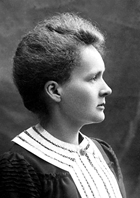
\includegraphics{Marie_Curie_1903}}
\caption{1903 Nobel Prize portrait}
\label{nobel_portrait_1903}
\end{figure}
\end{center}

\subsection{Nobel Prizes}

In December 1903, the Royal Swedish Academy of Sciences awarded Pierre Curie, Marie Curie and Henri Becquerel the Nobel Prize in Physics, ``in recognition of the extraordinary services they have rendered by their joint researches on the radiation phenomena discovered by Professor Henri Becquerel.'' At first, the Committee intended to honour only Pierre and Becquerel, but one of the committee members and an advocate of woman scientists, Swedish mathematician Magnus Goesta Mittag-Leffler, alerted Pierre to the situation, and after his complaint, Marie's name was added to the nomination. Marie was the first woman to be awarded a Nobel Prize.

Curie and her husband declined to go to Stockholm to receive the prize in person; they were too busy with their work, and Pierre, who disliked public ceremonies, was feeling increasingly ill. As Nobel laureates were required to deliver a lecture, the Curies finally undertook the trip in 1905. The award money allowed the Curies to hire their first lab assistant. Following the award of the Nobel Prize, and galvanised by an offer from the University of Geneva, which offered Pierre a position, the University of Paris gave Pierre a professorship and the chair of physics, although the Curies still did not have a proper laboratory. Upon Pierre's complaint, the University of Paris relented and agreed to furnish a new laboratory, but it would not be ready until 1906.

In December 1904, Curie gave birth to their second daughter, \'Eve. She later hired Polish governesses to teach her daughters her native language, and sent or took them on visits to Poland.

On 19 April 1906 Pierre was killed in a road accident. Walking across the Rue Dauphine in heavy rain, he was struck by a horse-drawn vehicle and fell under its wheels; his skull was fractured. Curie was devastated by her husband's death. On 13 May 1906 the physics department of the University of Paris decided to retain the chair that had been created for Pierre and to offer it to Marie. She accepted it, hoping to create a world-class laboratory as a tribute to Pierre. She was the first woman to become a professor at the University of Paris.

Curie's quest to create a new laboratory did not end with the University of Paris, however. In her later years, she headed the Radium Institute (Institut du radium, now Curie Institute, Institut Curie), a radioactivity laboratory created for her by the Pasteur Institute and the University of Paris. The initiative for creating the Radium Institute had come in 1909 from Pierre Paul \'Emile Roux, director of the Pasteur Institute, who had been disappointed that the University of Paris was not giving Curie a proper laboratory and had suggested that she move to the Pasteur Institute. Only then, with the threat of Curie leaving, did the University of Paris relent, and eventually the Curie Pavilion became a joint initiative of the University of Paris and the Pasteur Institute.

In 1910 Curie succeeded in isolating radium; she also defined an international standard for radioactive emissions that was eventually named for her and Pierre: the curie. Nevertheless, in 1911 the French Academy of Sciences did not elect her to be a member by one or two votes Elected instead was \'Edouard Branly, an inventor who had helped Guglielmo Marconi develop the wireless telegraph. A doctoral student of Curie, Marguerite Perey, became the first woman elected to membership in the Academy - over half a century later, in 1962. Despite Curie's fame as a scientist working for France, the public's attitude tended toward xenophobia-the same that had led to the Dreyfus affair-which also fuelled false speculation that Curie was Jewish. During the French Academy of Sciences elections, she was vilified by the right wing press, who criticised her for being a foreigner and an atheist. Her daughter later remarked on the public hypocrisy; as the French press often portrayed Curie as an unworthy foreigner when she was nominated for a French honour, but would portray her as a French hero when she received a foreign one, such as her Nobel Prizes.

In 1911, it was revealed that in 1910-11 Curie had conducted an affair of about a year's duration with physicist Paul Langevin, a former student of Pierre's. He was a married man who was estranged from his wife. This resulted in a press scandal that was exploited by her academic opponents. Curie (then in her mid-40s) was five years older than Langevin and was portrayed in the tabloids as a foreign Jewish home-wrecker. She was away for a conference in Belgium when the scandal broke; upon her return, she found an angry mob in front of her house, and had to seek a refuge, with her daughters, at a house of a friend.

International recognition for her work had been growing to new heights, and the Royal Swedish Academy of Sciences honoured her a second time, with the 1911 Nobel Prize in Chemistry. This award was ``in recognition of her services to the advancement of chemistry by the discovery of the elements radium and polonium, by the isolation of radium and the study of the nature and compounds of this remarkable element.'' She was the first person to win or share two Nobel Prizes, and remains alone with Linus Pauling as Nobel laureates in two fields each. A delegation of celebrated Polish men of learning, headed by novelist Henryk Sienkiewicz, encouraged her to return to Poland and continue her research in her native country. Curie's second Nobel Prize enabled her to talk the French government into supporting the Radium Institute, which was built in 1914 and at which research was conducted in chemistry, physics, and medicine. A month after accepting her 1911 Nobel Prize, she was hospitalised with depression and a kidney ailment. For most of 1912, she avoided public life, and spent some time in England with her friend and fellow physicist, Hertha Ayrton. She returned to her lab only in December, after a break of about 14 months.

In 1912, the Warsaw Scientific Society offered her the directorship of a new laboratory in Warsaw, but she declined, focusing on the developing Radium Institute, to be completed in August 1914 and a new street named Rue Pierre-Curie. She visited Poland in 1913, and was welcomed in Warsaw, but the visit was mostly ignored by the Russian authorities. The Institute's development was interrupted by the coming war, as most researchers were drafted into the French Army, and it fully resumed its activities in 1919.

\subsection{Death} 
Curie visited Poland for the last time in early 1934. A few months later, on 4 July 1934, she died at the Sancellemoz Sanatorium in Passy, in Haute-Savoie, from aplastic anemia believed to have been contracted from her long-term exposure to radiation. The damaging effects of ionising radiation were not known at the time of her work, which had been carried out without the safety measures later developed. She had carried test tubes containing radioactive isotopes in her pocket and stored them in her desk drawer, remarking on the faint light that the substances gave off in the dark. Curie was also exposed to X-rays from unshielded equipment while serving as a radiologist in field hospitals during the war. Although her many decades of exposure to radiation caused chronic illnesses (including near blindness due to cataracts) and ultimately her death, she never really acknowledged the health risks of radiation exposure.

She was interred at the cemetery in Sceaux, alongside her husband Pierre. Sixty years later, in 1995, in honour of their achievements, the remains of both were transferred to the Panth\'eon, Paris. She became the first-and so far the only-woman to be honoured with interment in the Panth\'eon on her own merits.

Because of their levels of radioactivity, her papers from the 1890s are considered too dangerous to handle. Even her cookbook is highly radioactive. Her papers are kept in lead-lined boxes, and those who wish to consult them must wear protective clothing.

In her last year she worked on a book, Radioactivity, which was published posthumously in 1935.


\section{Legacy} 
The physical and societal aspects of the Curies' work contributed substantially to shaping the world of the twentieth and twenty-first centuries. Cornell University professor L. Pearce Williams observes:

    The result of the Curies' work was epoch-making. Radium's radioactivity was so great that it could not be ignored. It seemed to contradict the principle of the conservation of energy and therefore forced a reconsideration of the foundations of physics. On the experimental level the discovery of radium provided men like Ernest Rutherford with sources of radioactivity with which they could probe the structure of the atom. As a result of Rutherford's experiments with alpha radiation, the nuclear atom was first postulated. In medicine, the radioactivity of radium appeared to offer a means by which cancer could be successfully attacked.

If Marie Curie's work helped overturn established ideas in physics and chemistry, it has had an equally profound effect in the societal sphere. To attain her scientific achievements, she had to overcome barriers that were placed in her way because she was a woman, in both her native and her adoptive country. This aspect of her life and career is highlighted in Fran\c{c}oise Giroud's Marie Curie: A Life, which emphasises Marie's role as a feminist precursor.

She was known for her honesty and moderate life style. Having received a small scholarship in 1893, she returned it in 1897 as soon as she began earning her keep. She gave much of her first Nobel Prize money to friends, family, students and research associates. In an unusual decision, Marie intentionally refrained from patenting the radium-isolation process, so that the scientific community could do research unhindered. She insisted that monetary gifts and awards be given to the scientific institutions she was affiliated with rather than to herself. She and her husband often refused awards and medals. Albert Einstein reportedly remarked that she was probably the only person who could not be corrupted by fame.

\section{Awards, honours and tributes}

As one of the most famous female scientists to date, Marie Curie has become an icon in the scientific world and has received tributes from across the globe, even in the realm of pop culture. In a 2009 poll carried out by New Scientist, Marie Curie was voted the ``most inspirational woman in science''. Curie received 25.1 per cent of all votes cast, nearly twice as many as second-place Rosalind Franklin (14.2 per cent).

Poland and France declared 2011 the Year of Marie Curie, and the United Nations declared that this would be the International Year of Chemistry. An artistic installation celebrating ``Madame Curie'' filled the Jacobs Gallery at San Diego's Museum of Contemporary Art. On 7 November, Google celebrated her birthday with a special Google Doodle. On 10 December, the New York Academy of Sciences celebrated the centenary of Marie Curie's second Nobel prize in the presence of Princess Madeleine of Sweden.

Marie Curie was the first woman to win a Nobel prize, the first person to win two Nobel Prizes, the only woman to win in two fields, and the only person to win in multiple sciences. Awards that she received include:

\begin{itemize}
\item{Nobel Prize in Physics (1903)}
\item{Davy Medal (1903, with Pierre)}
\item{Matteucci Medal (1904; with Pierre)}
\item{Elliott Cresson Medal (1909)}
\item{Nobel Prize in Chemistry (1911)}
\item{Franklin Medal of the American Philosophical Society (1921)}
\end{itemize}

In 1995, she became the first woman to be entombed on her own merits in the Panth\'eon, Paris. The curie (symbol Ci), a unit of radioactivity, is named in honour of her and Pierre (although the commission which agreed on the name never clearly stated whether the standard was named after Pierre, Marie or both of them). The element with atomic number 96 was named curium. Three radioactive minerals are also named after the Curies: curite, sklodowskite, and cuprosklodowskite. She received numerous honorary degrees from universities across the world. The Marie Curie Actions fellowship program of the European Union for young scientists wishing to work in a foreign country is named after her. In Poland, she had received honorary doctorates from the Lw\'ow Polytechnic (1912), Pozna\'n University (1922), Krak\'ow's Jagiellonian University (1924), and the Warsaw Polytechnic (1926).

Numerous locations around the world are named after her. In 2007, a metro station in Paris was renamed to honour both of the Curies. Polish nuclear research reactor Maria is named after her. The 7000 Curie asteroid is also named after her. A KLM McDonnell Douglas MD-11 (registration PH-KCC) is named in her honour.
2011 birthplace mural, on centenary of second Nobel Prize

Several institutions bear her name, starting with the two Curie institutes - the Maria Sk\l{}odowska-Curie Institute of Oncology, in Warsaw; and the Institut Curie in Paris. She is the patron of Maria Curie-Sk\l{}odowska University, in Lublin, founded in 1944; and of Paris' Pierre and Marie Curie University, established 1971. In Britain, Marie Curie Cancer Care was organised in 1948 to care for the terminally ill.

Two museums are devoted to Marie Curie. In 1967, the Maria Sk\l{}odowska-Curie Museum was established in Warsaw's ``New Town'', at her birthplace on ulica Freta (Freta Street). Her Paris laboratory is preserved as the Mus\'ee Curie, open since 1992.

Several works of art bear her likeness. In 1935, Michalina Mo\'scicka, wife of Polish President Ignacy Mo\'scicki, unveiled a statue of Marie Curie before Warsaw's Radium Institute. During the 1944 Second World War Warsaw Uprising against the Nazi German occupation, the monument was damaged by gunfire; after the war it was decided to leave the bullet marks on the statue and its pedestal. In 1955 Jozef Mazur created a stained glass panel of her, the Maria Sk\l{}odowska-Curie Medallion, featured in the University at Buffalo Polish Room.

A number of biographies are devoted to her. In 1938 her daughter, \'Eve Curie, published Madame Curie. In 1987 Fran\c{c}oise Giroud wrote Marie Curie: A Life. In 2005 Barbara Goldsmith wrote Obsessive Genius: The Inner World of Marie Curie. In 2011 Lauren Redniss published Radioactive: Marie and Pierre Curie, a Tale of Love and Fallout .

Greer Garson and Walter Pidgeon starred in the 1943 U.S. Oscar-nominated film, Madame Curie, based on her life. More recently, in 1997, a French film about Pierre and Marie Curie was released, Les Palmes de M. Schutz. It was adapted from a play of the same name. In the film, Marie Curie was played by Isabelle Huppert.

Curie is the subject of the play False Assumptions by Lawrence Aronovitch, in which the ghosts of three other female scientists observe events in her life.

Curie's likeness also has appeared on bills, stamps and coins around the world. She was featured on the Polish late-1980s 20,000-z\l{}oty banknote as well as on the last French 500-franc note, before the franc was replaced by the euro.

On the 2011 centenary of Marie Curie's second Nobel Prize (1911), an allegorical mural was painted on the fa\c{c}ade of her Warsaw birthplace. It depicts an infant Maria Sk\l{}odowska holding a test tube from which emanate the elements that she would discover as an adult: polonium and radium.

\bibliographystyle{chicago}
\bibliography{marie_curie_wiki}
\end{document} 

